\chapter{Results}

\section{Mean Field Results}

Several calibrated relativistic mean field models are used to predict the point-nuclear form factors for various nuclei of interest. The noble gases, Argon-40 and Xenon-132 are studied because of their continued interest and applicability for dark matter detectors~\cite{schumann:2012:dark}. Iodine-127 and Cesium-133 are studied because of their use in the recent experimental achievement to measure \cevns . The formalism provided in this report is particularly geared towards spinless, symmetric nuclei, namely, even number of protons and neutrons. Pairing effects due to the unpaired nucleons and deformation of the nucleus are not accounted for. This is important to mention because Iodine-127 and Cesium-133 have an uneven number of protons. The contributions from the unpaired proton in Iodine-127 and Cesium-133 need to be further studied. Showing the similarities of the density distributions of Xenon to that of Cesium and Iodine in this report gives us some quantitative evidence that the effects due to the unpaired proton are minimal. 

Taking the IFT of the nuclear form factor yields the density distribution for point-nucleons as discussed in Subsection~\ref{sec:nuclearff}. From the density distributions the root-mean-square radii are calculated using~\eqref{eq:rootmean}, i.e., $R=\sqrt{\langle r^2 \rangle}$. The predicted values for the root-mean-square radii are shown in Table~\ref{table:radii} on page~\pageref{table:radii}. The models used in this report have been chosen by analyzing the neutron skin, $R_n-R_p$, of Lead-208. Moreover, the models that gave a wide range of values for the neutron skin were chosen to reflect a wide range of predicted values for the radius of the neutron distribution.

% Proton and Neutron Densities
\begin{figure}
\centering
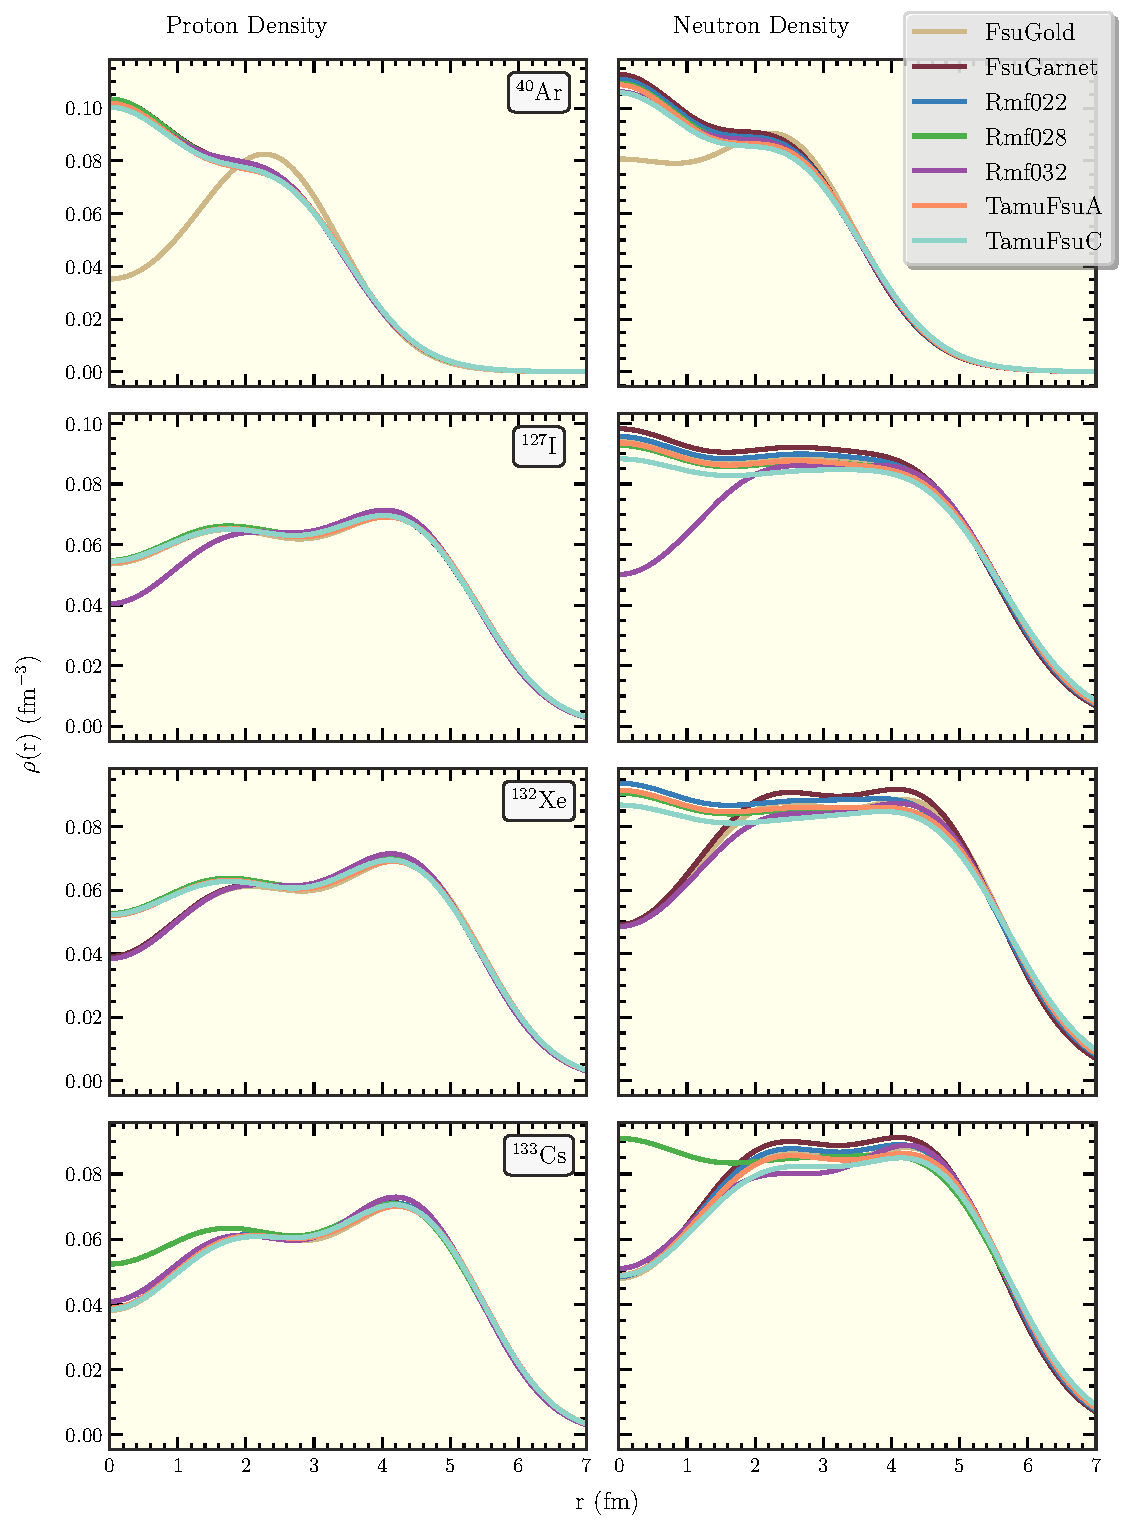
\includegraphics[width=\textwidth, height=0.9\textheight]{figures/proton_neutron_den}
\caption{Point-nuclear density distributions are calculated using the models listed. Each row shares the y-axes and corresponds to a given nucleus as labeled. The first and second columns share the x-axes and represent the proton and neutron distributions respectively.}
\label{fig:pointnucden}
\end{figure}

Using the nuclear mean-field potentials~\eqref{eq:meanpot} for the ground state nucleus and solving the coupled first order Dirac equations,~\eqref{eq:diracsingles}, produced the result for the Dirac spinors, namely, the lower and upper component bound-state wave functions. In addition, the lower and upper wave functions are used the calculate the proton and neutron density distributions using~\eqref{eq:nuclearden}. Figure~\ref{fig:pointnucden} shows the results of calculating the neutron and proton densities for the four nuclei of interest in this study. 

The model predictions for the radius of the proton distributions agree within $\sim 1\% $ with the experimental values; this reflects the fact that our models for the proton distributions are well constrained by experiment. In contrast, one can see that the neutron distributions have much greater deviations depending on the model because it is much less constrained. In other words the isoscalar sector of the interaction is well understood through various hadronic probes as discussed in~\ref{sec:nuclearmot}. On the contrary, the isovector sector of the weak interaction is not well understood; \cevns\ will allow the isovector sector parameters to be  much better constrained. 

The density distributions that tend to have a lower value at the origin, commonly called a `hole', is due to the model choice of occupied energy levels. The behavior of the wave function at the origin goes like $\sim r^{l+1}$ , therefore, is dominated by the $l=0$ bound-state energy solutions. This is due to the linear behavior at the origin of the wave functions for $l=0$ states, compared to a slower increase at the origin for higher orbital angular momentum. The subtlety of the `hole' comes from the fact that the energy levels are almost degenerate with differences in energies on the order of an MeV to keV for the shell closure. For example, FsuGold model predicts a `hole' for the proton density distribution because the $D_{5/2}$ orbital has a lower energy than the $S_{1/2}$ and thus closes the shell. 

The mean-field density predictions are used to calculate the point-nucleon form factors by taking the FT using~\eqref{eq:pointnuclearff}. These results will be used to compute the experimentally accessible charge and weak form factors in the next Section.

\section{Experimentally Accessible Results}

The experimentally accessible quantities pertinent to this study come in the form of the charge and weak nuclear form factor and the \cevns\ cross section discussed in Section~\ref{sec:cevnsform}. 

\subsection{Form Factor}
As discussed in the previous section the Fourier transform of the nuclear densities of the point-nucleons of Figure~\ref{fig:pointnucden} can be used to obtain the nuclear form factors. Using~\eqref{eq:chwkFF}, the nuclear form factors are folded with the single-nucleon electric Sachs form factors of Figure~\ref{fig:singlenucleonFF}; Figure~\ref{fig:nuclearlogff} shows the results of this procedure.
%charge and weak ff
\begin{figure}
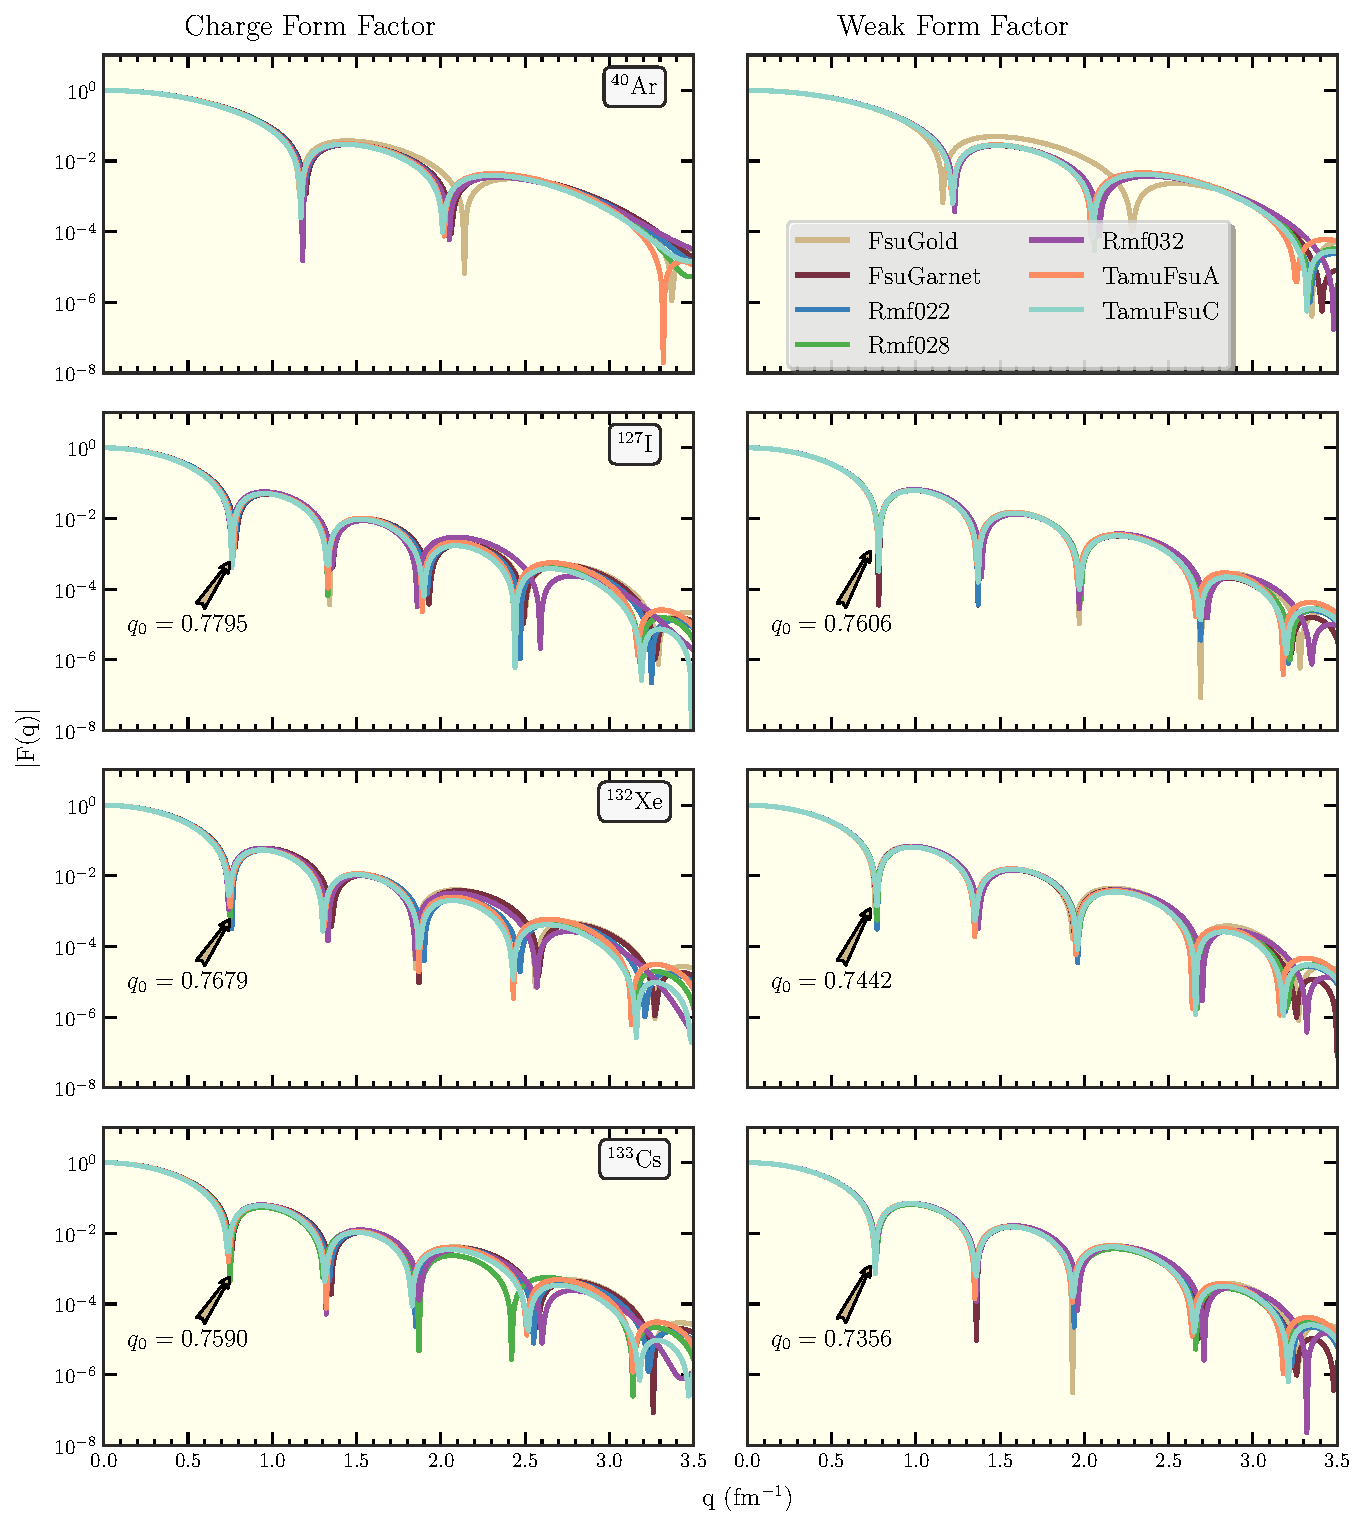
\includegraphics[width=\textwidth, height=0.9\textheight]{figures/nuclearlogFF}
\caption{Nuclear charge and weak form factors from folding the single-nucleon form factors with the point-nuclear form factors. The columns and rows follow the same procedure as Figure~\ref{fig:pointnucden}.}
\label{fig:nuclearlogff}
\end{figure}
The absolute value of the form factor, $|F(q)|$, is taken in order to show the oscillatory behavior on a log plot. This procedure allows for the diffraction minimum of the form factor to be seen. These `dips' are characteristic minimum values of the form factor at specific momentum transfer due to the oscillations at larger $q$-values. Note that the minimum $q$-values increase in frequency and shift to slightly smaller values for larger and more neutron rich nuclei; the first minimum value, $q_0$, is shown in Figure~\ref{fig:nuclearlogff} for the heavier elements. At small momentum transfer the form factor is almost model independent. Comparing the weak and charge form factors, it can be seen that momentum transfers where the minima in the form factor occur are slightly smaller. The minima of the form factors occur at slightly smaller momentum transfer for heavier nuclei because the exponential decay of the form factor is dominated by the mean-squared radius of the density distribution. 

%From the behavior of exponential decay of the form factor is characteristic of the diffuseness of the nuclei, namely, the the distance from the central value to that which the nuclear density becomes small. It is evident that most of the model predictions agree with the minimum momentum transfer with deviations at larger values. Comparing the weak and charge form factors, it can be seen that the minimum values of momentum transfer are slightly smaller for the weak form factors. This is due to the neutron richness and reflects the fact that the weak mean-squre radii are larger than the charge radii. 

Figure~\ref{fig:pbweakFF} shows that our results using various relativistic mean field models agree fairly well with the parity violating electron scattering experiment done by the PREX collaboration~\cite{PREX:2012:measurementPb}. From the data the form factor was extracted at a value of $\bar{q}=0.475$ fm$^{-1}$ with a weak radius of $R_w=5.836(182)$ where the model and experimental errors are added in quadrature. This figure also illuminates the extreme difficulty and sensitivity needed in the experiments to constrain the  models. In order to differentiate the theoretical models the error bars need to be reduced to $\sim 0.1\%$ error. 
%Another interesting feature that is important to note is the fact that the theoretical results are all greater than the experimental results. Furthermore, the fact that the theoretical results are greater would indicate that the true situation in nature seems to point towards a reduction in the present mean field approach.

%talk about diffusness and decay
\begin{figure}
\centering
\includegraphics[scale=0.9, keepaspectratio]{figures/Pb208_weakFF}
\caption{The weak form factor of $^{208}$Pb for various models and the experimentally extracted weak form factor from parity violating electron scattering experiment, PREX~\cite{PREX:2012:measurementPb}. The inset zooms in on the experimental point to compare our results.}
\label{fig:pbweakFF}
\end{figure}
%charge and weak densities
\begin{figure}
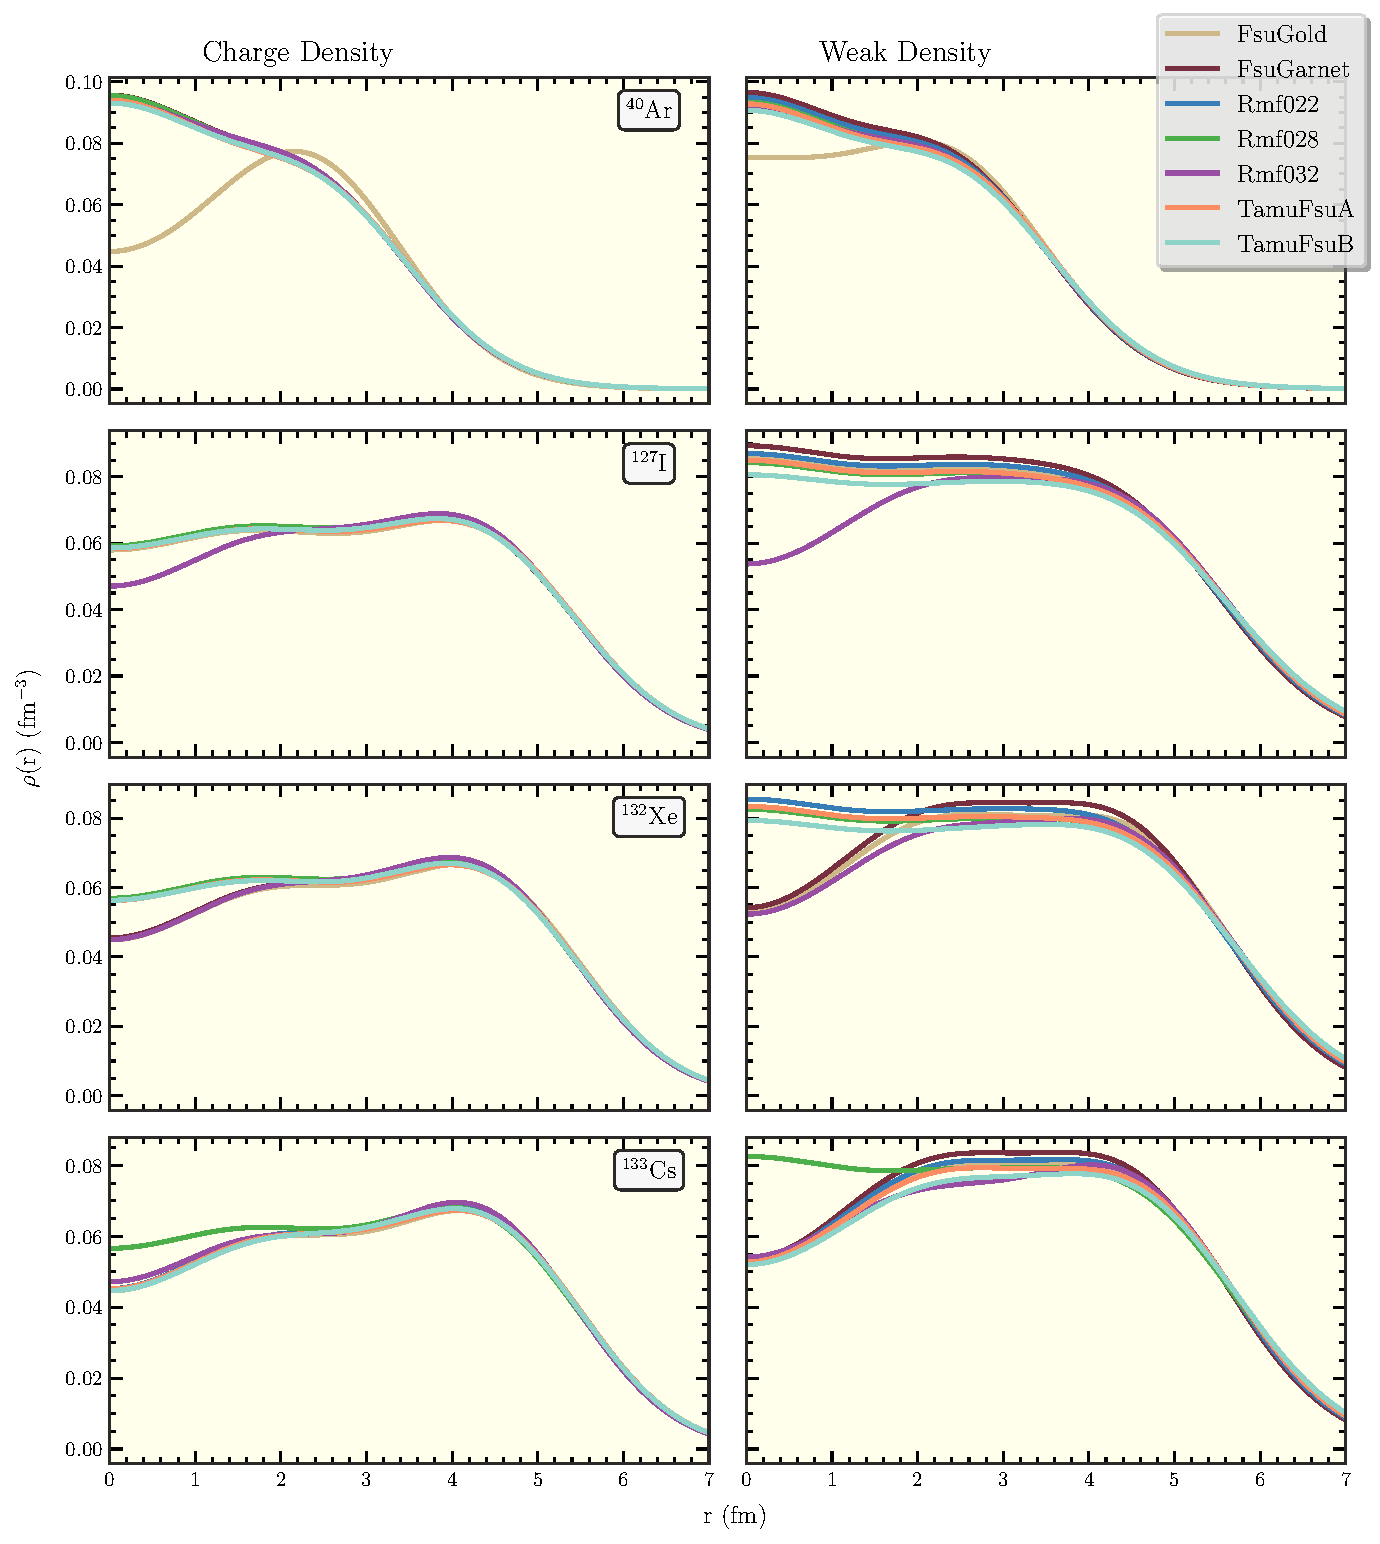
\includegraphics[width=\textwidth, height=0.9\textheight]{figures/nuclearden}
\caption{Nuclear charge and weak density distributions calculated from the charge and weak form factors for the models shown. The columns and rows follow the same procedure as Figure~\ref{fig:pointnucden}.}
\label{fig:nuclearden}
\end{figure} 

Figure~\ref{fig:nuclearden} shows the charge and weak density obtained from taking the FT of the respective form factor after folding with the single nucleon form factors.

Comparison of the point-nuclear density distributions with the charge and weak density distribution shows almost identical results. This confirms, as it should be, that the charge distribution is almost entirely sensitive to the distribution of protons and the weak distribution are conversely sensitive to the neutrons in the nucleus. This is a result of the charge of the protons and the weak charge of the neutrons. The charge of the protons couples very strongly to the electromagnetic interaction, where the neutrons are neutral. Conversely, the neutrons couple very strongly to the weak interaction and the protons have almost no weak charge. 

To gain a better understanding of the form factor we can introduce an analytic form of the form factor using the symmetrized Fermi function described in full detail in Ref~\cite{piekarewicz:2016:power}. The form factor for the spherically symmetric nuclei using the symmetrized Fermi density is given as:
\begin{equation}\label{eq:symff}
F_{sf}(q) = \frac{3\pi a}{qc[c^2+\pi ^2 a^2]}\left[ \frac{1}{\sinh \pi qa}\right] \left[\frac{\pi a}{\tanh\pi qa}\sin qc - c\cos qc\right],
\end{equation}
where $a$ and $c$ are the so called surface diffuseness and half-density radius respectively; better known from the Fermi density $\rho (r)=\frac{\rho _0}{1+e^{(r-c)/a}}$. Taking~\eqref{eq:symff} at large momentum transfer yields:
\begin{equation}
F_{sf} \Longrightarrow -\frac{6\pi a}{\sqrt{c^2+\pi ^2 a^2}}\frac{\cos(qc+\beta )}{qc}e^{-\pi q a},\quad \text{where}\quad 
\beta = \tan ^{-1} \frac{\pi a}{c},
\end{equation}
where asymptotically $\sinh x \rightarrow\frac{e^x}{2}$, $\tanh x\rightarrow 1$ and the trigonometric identity, $-\cos (\alpha +\beta)= \sin\alpha \sin\beta - \cos\alpha \cos\beta$, have been used. One can see clearly from the asymptotic form of~\eqref{eq:symff} that the exponential decay of the form factor is due to the surface diffuseness, $a$, and the oscillations are controlled by the half-density radius, $c$.

Qualitative analysis of the density distributions show how the half-density and surface diffuseness affect the form factors. Comparing the density distributions for Argon-40 and the heavier nuclei one can see that the half-density parameter is smaller. For smaller nuclei the form factor has fewer oscillations and they begin at higher descent indicative of a smaller half-density. The surface diffuseness indicates how steep the decent of the density distributions are and translates to the rate of exponential decay in the form factor. From this quantitative analysis it is shown that the heavier nuclei have larger surface diffuseness and half-density distances leading to larger exponential decay and oscillations at smaller $q$-values.

\begin{figure}[t!]%Weak Skin Form factor
\centering
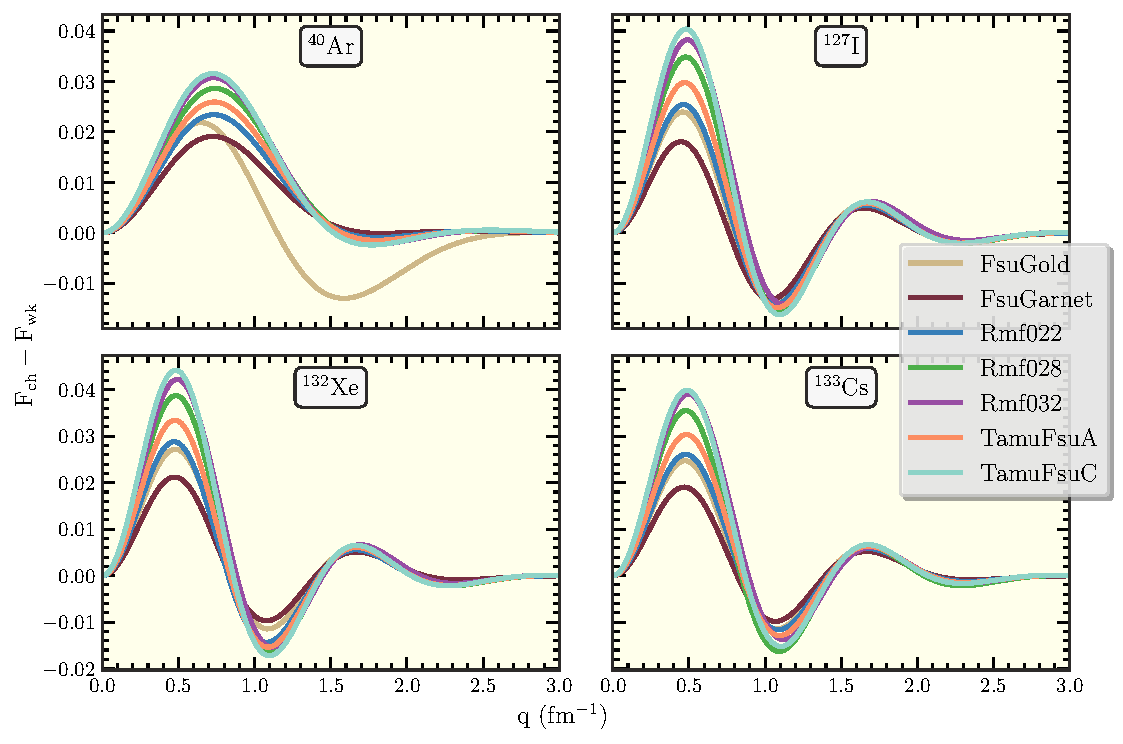
\includegraphics[width=1\textwidth]{figures/charge_weak_FF}
\caption{The nuclear weak skin form factor, $F_{ch}-F_w$, is shown for all the models used in this report.}
\label{fig:wkff}
\end{figure}
The weak skin form factor can be constructed by subtracting the charge form factor from the weak form factor distributions,~\eqref{fig:nuclearlogff}. Taking the form factor expansion,~\eqref{eq:expandff}, to the first moment gives us an approximate form for the weak skin, namely,
\begin{align}
F_{ch}(Q^2)-F_w(Q^2) &\approx (1-\frac{Q^2}{6}R_{ch}^2)-(1-\frac{Q^2}{6}R_w^2) \nonumber \\
&= \frac{Q^2}{6}(R_w^2-R_{ch}^2) \nonumber \\
&= \frac{Q^2}{6}(R_w+R_{ch})(R_w-R_{ch}).\label{eq:wkskinff}
\end{align}
In~\eqref{eq:wkskinff} the weak skin form factor, $F_{ch}-F_w$, is directly proportional to the weak skin, $R_w-R_{ch}$. This is of great importance for experimental analysis because the weak and charge form factor are what is measured directly. With this formalism the weak skin may be extracted in a model-independent way. The weak skin form factor is shown for the four studied nuclei in Figure~\ref{fig:wkff}. From Figure~\ref{fig:wkff}, it can be seen that the curvature near the origin and the peaks of the form factor are controlled by the weak skin. Furthermore, the slope of the weak form factor is larger for the more neutron rich matter and the models with larger weak skin have greater peaks, as they should.   

From the density distributions one can extract the root-mean-square radius as discussed earlier. Experimentally the root-mean-square radius is extracted from the first even moment of the form factor expansion as discussed in Subsection~\ref{sec:nuclearff}. Specifically, the charge radius of many nuclei have been extensively researched and are very well known. It is shown that our models agree very well with the experimental charge radii of the nuclei of study by comparing the calculated and experimental values in Table~\ref{table:radii}. Note that for a particular nucleus the proton and charge radii are fairly consistent. In contrast, the neutron distributions are poorly known and the neutron and weak radii vary largely from model to model. One can see the experimental results of the charge root-mean-square radii and some initial experimental values for the neutron and weak radii to compare with our results. The experimental rows of Table~\ref{table:radii} show charge radius results from a combination of muonic spectra and electron scattering data~\cite{angeli:2013:table}, recent results for Calcium-40 and Calcium-48 of the neutron skin~\cite{zenihiro:2018:direct} using proton scattering with hadronic model dependent errors, and weak neutron radius of Lead-208 from parity violating electron scattering~\cite{PREX:2012:measurementPb}. 
%Calculated Radii
\def\arraystretch{1.1}
\setlength\LTleft{0pt}
\setlength\LTright{0pt}
\begin{longtable}{@{\extracolsep{\fill}}r || c | *{3}{c} | *{3}{c}}
\caption{Theoretically calculated root-mean-squared radii from the seven relativistic mean field models, showing the neutron and proton radii, neutron skins, charge and weak radii, and weak skins extracted from the predicted density distributions.} \label{table:radii}\\
\hline\hline
Nucleus & Model & $R_p$ & $R_n$ & $R_n-R_p$ & $R_{ch}$ & $R_w$ & $R_w-R_{ch}$ 
\\ \hline 
\endfirsthead 
\caption*{Table~\ref{table:radii} - continued}\\ 
\hline\hline
Nucleus & Model & $R_p$ & $R_n$ & $R_n-R_p$ & $R_{ch}$ & $R_w$ & $R_w-R_{ch}$\\ \hline 
\endhead
\hline\hline 
\endfoot
$^{40}\mathrm{Ca}$ & FsuGold & 3.337 & 3.286 & -0.0512 & 3.426 & 3.372 & -0.0538 \\
 & FsuGarnet & 3.345 & 3.292 & -0.0522 & 3.433 & 3.378 & -0.0548 \\
 & Rmf022 & 3.351 & 3.299 & -0.0517 & 3.439 & 3.385 & -0.0543 \\
 & Rmf028 & 3.350 & 3.300 & -0.0495 & 3.438 & 3.386 & -0.0520 \\
 & Rmf032 & 3.357 & 3.309 & -0.0479 & 3.445 & 3.395 & -0.0503 \\ 
 & TamuFsuA & 3.358 & 3.307 & -0.0501 & 3.446 & 3.393 & -0.0527 \\
 & TamuFsuC & 3.374 & 3.329 & -0.0455 & 3.462 & 3.414 & -0.0478 \\ 
\hline 
 & Experiment~\cite{ angeli:2013:table, zenihiro:2018:direct} & 3.385 & 3.375 & 0.010$^{+0.048}_{-0.049}$ & 3.4776(19) &  & 
\\ \hline
$^{40}\mathrm{Ar}$ & FsuGold & 3.253 & 3.363 & 0.1106 & 3.343 & 3.459 & 0.1166 \\
 & FsuGarnet & 3.269 & 3.350 & 0.0807 & 3.358 & 3.444 & 0.0857 \\
 & Rmf022 & 3.270 & 3.367 & 0.0970 & 3.359 & 3.462 & 0.1026 \\
 & Rmf028 & 3.266 & 3.382 & 0.1156 & 3.355 & 3.477 & 0.1217 \\
 & Rmf032 & 3.266 & 3.393 & 0.1269 & 3.355 & 3.489 & 0.1334 \\
 & TamuFsuA & 3.277 & 3.383 & 0.1058 & 3.366 & 3.478 & 0.1116 \\
 & TamuFsuC & 3.282 & 3.414 & 0.1318 & 3.371 & 3.510 & 0.1385 \\ 
\hline 
 & Experiment~\cite{angeli:2013:table} &  &  &  & 3.4274(29) &  & \\
\hline
$^{48}\mathrm{Ca}$ & FsuGold & 3.365 & 3.562 & 0.1972 & 3.451 & 3.657 & 0.2063 \\
 & FsuGarnet & 3.365 & 3.563 & 0.1971 & 3.451 & 3.658 & 0.2062 \\
 & Rmf022 & 3.356 & 3.553 & 0.1966 & 3.442 & 3.648 & 0.2056 \\
 & Rmf028 & 3.352 & 3.584 & 0.2315 & 3.438 & 3.680 & 0.2415 \\
 & Rmf032 & 3.345 & 3.589 & 0.2438 & 3.432 & 3.686 & 0.2541 \\
 & TamuFsuA & 3.366 & 3.581 & 0.2144 & 3.452 & 3.676 & 0.2240 \\
 & TamuFsuC & 3.366 & 3.616 & 0.2501 & 3.452 & 3.713 & 0.2606 \\ \hline 
 & Experiment~\cite{angeli:2013:table, zenihiro:2018:direct} & 3.387 & 3.555 & 0.168$^{+0.052}_{-0.055}$ & 3.4771(22) &  &  \\
\hline
$^{127}\mathrm{I}$ & FsuGold & 4.665 & 4.830 & 0.1646 & 4.727 & 4.901 & 0.1739 \\
 & FsuGarnet & 4.655 & 4.785 & 0.1305 & 4.717 & 4.856 & 0.1384 \\  
 & Rmf022 & 4.650 & 4.821 & 0.1717 & 4.712 & 4.893 & 0.1811 \\  
 & Rmf028 & 4.640 & 4.862 & 0.2221 & 4.703 & 4.936 & 0.2335 \\  
 & Rmf032 & 4.637 & 4.872 & 0.2345 & 4.700 & 4.946 & 0.2464 \\  
 & TamuFsuA & 4.660 & 4.855 & 0.1952 & 4.722 & 4.928 & 0.2056 \\  
 & TamuFsuC & 4.655 & 4.913 & 0.2575 & 4.718 & 4.988 & 0.2703 \\ 
\hline
 & Experiment~\cite{angeli:2013:table} &  &  &  & 4.7500(81) &  &
\\ \hline
$^{132}\mathrm{Xe}$ & FsuGold & 4.713 & 4.885 & 0.1714 & 4.775 & 4.956 & 0.1809 \\ 
 & FsuGarnet & 4.692 & 4.829 & 0.1368 & 4.754 & 4.899 & 0.1449 \\ 
 & Rmf022 & 4.690 & 4.879 & 0.1884 & 4.752 & 4.951 & 0.1985 \\ 
 & Rmf028 & 4.683 & 4.925 & 0.2420 & 4.745 & 4.999 & 0.2541 \\ 
 & Rmf032 & 4.679 & 4.935 & 0.2557 & 4.741 & 5.009 & 0.2682 \\
 & TamuFsuA & 4.703 & 4.916 & 0.2136 & 4.764 & 4.989 & 0.2247 \\
 & TamuFsuC & 4.6991 & 4.976 & 0.2776 & 4.760 & 5.051 & 0.2910 \\ 
\hline
 & Experiment~\cite{angeli:2013:table} &  &  &  & 4.7859(52) &  & \\ 
\hline
$^{133}\mathrm{Cs}$ & FsuGold & 4.733 & 4.891 & 0.1580 & 4.795 & 4.962 & 0.1670 \\
 & FsuGarnet & 4.713 & 4.838 & 0.1251 & 4.774 & 4.907 & 0.1329  \\
 & Rmf022 & 4.712 & 4.877 & 0.1646 & 4.774 & 4.948 & 0.1738 \\
 & Rmf028 & 4.705 & 4.930 & 0.2243 & 4.767 & 5.003 & 0.2358 \\
 & Rmf032 & 4.695 & 4.927 & 0.2322 & 4.757 & 5.001 & 0.2440 \\
 & TamuFsuA & 4.727 & 4.915 & 0.1877 & 4.789 & 4.986 & 0.1979 \\
 & TamuFsuC & 4.723 & 4.968 & 0.2444 & 4.785 & 5.042 & 0.2567 \\ 
\hline
& Experiment~\cite{angeli:2013:table} &  &  &  & 4.8041(46) &  & \\ 
\hline
$^{208}\mathrm{Pb}$ & FsuGold & 5.465 & 5.669 & 0.2043 & 5.518 & 5.733 & 0.2150 \\
 & FsuGarnet & 5.437 & 5.597 & 0.1593 & 5.491 & 5.659 & 0.1684 \\
 & Rmf022 & 5.434 & 5.648 & 0.2138 & 5.487 & 5.712 & 0.2250 \\
 & Rmf028 & 5.431 & 5.713 & 0.2816 & 5.485 & 5.780 & 0.2952 \\
 & Rmf032 & 5.427 & 5.743 & 0.3162 & 5.480 & 5.811 & 0.3311 \\
 & TamuFsuA & 5.449 & 5.696 & 0.2470 & 5.502 & 5.762 & 0.2593 \\
 & TamuFsuC & 5.447 & 5.774 & 0.3267 & 5.500 & 5.842 & 0.3420 \\ 
\hline
& Experiment~\cite{angeli:2013:table, horowitz:2012:weak} & 5.449 & 5.751 & 0.302(177) & 5.5012(13) & 5.826 & 0.323(183) 
\\ 
\end{longtable}



%radii correlations
%\begin{figure}
%\centering
%\begin{subfigure}{.5\textwidth}
%  \centering
%  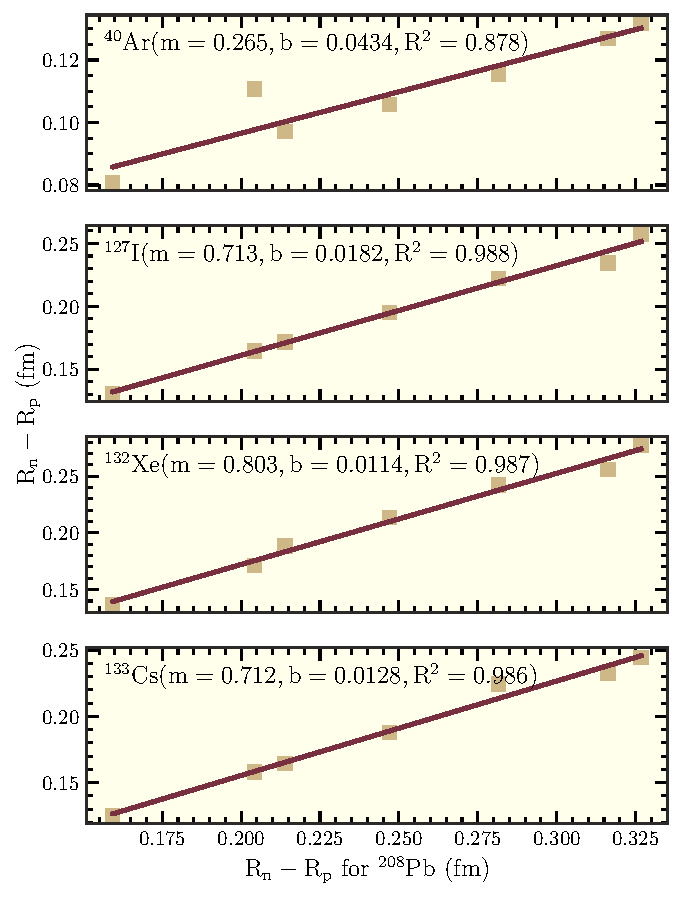
\includegraphics[width=1\linewidth]{figures/neutron_radius_corr}
%\end{subfigure}%
%\begin{subfigure}{.5\textwidth}
%  \centering
%  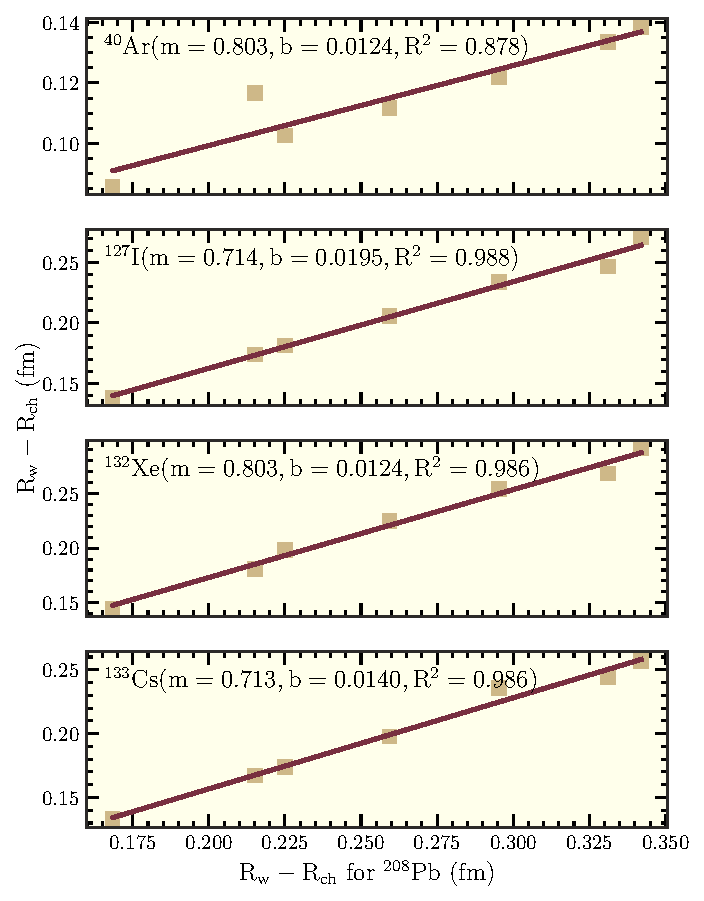
\includegraphics[width=1\linewidth]{figures/weak_radius_corr}
%\end{subfigure}
%\caption{A figure with two subfigures}
%\label{fig:test}
%\end{figure}

%model radii table

\subsection{Cross Section}

The \cevns\ cross section can be computed once the weak nuclear form factor is known using~\eqref{eq:totcross} as discussed in Subsection~\ref{sec:evalcross}. Figure~\ref{fig:nuccross} shows both the differential and total cross section for various nuclei using the FsuGold model. The differential cross section is taken at the energy of a monochromatic neutrino from pion decay at rest. This two-body decay of the form, $\pi ^+ \rightarrow \mu ^+ + \nu _{\mu} $, produces the monochromatic neutrino energy at 29.9~MeV~\cite{scholberg:2018:observation}. Incidentally, the value of the monochromatic neutrino energy from the pion decay at rest quoted in~\cite{scholberg:2018:observation} was a typo; the correct value for the neutrino energy is 29.792 MeV. The maximum nuclear recoil is determined by the mass of the target nuclei and incoming neutrino energy. It is evident that the target material has competing components, namely the number of neutrons and the recoil energy. As discussed in Chapter~\ref{chap:intro} the enhancement to the differential cross section for larger neutron rich nuclei is offset by the threshold that the nuclear recoil energy can be detected.

\begin{figure}
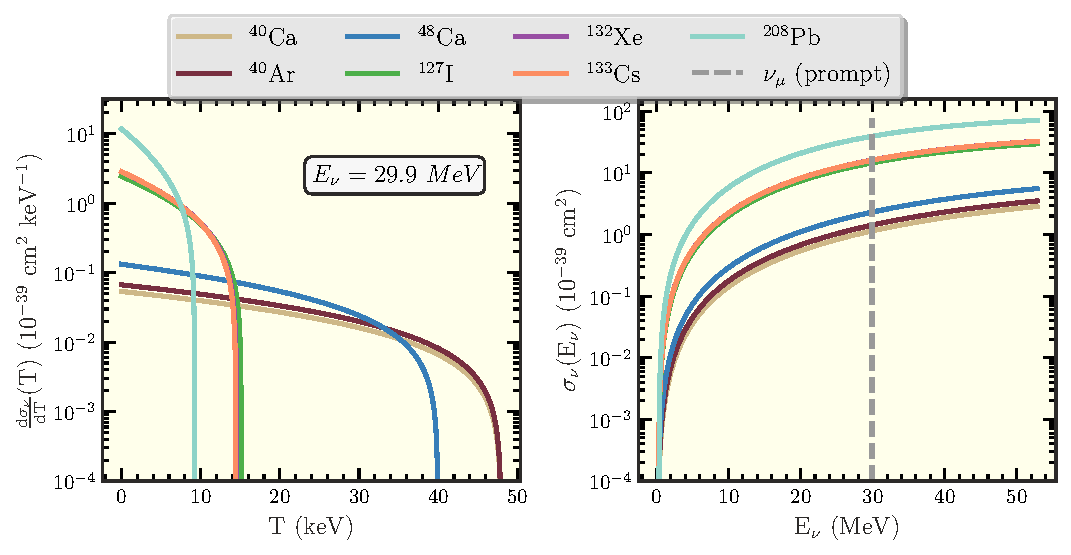
\includegraphics[width=1\textwidth, keepaspectratio]{figures/nuclearcross}
\caption{(\textbf{Left}) The differential cross-section as a function of nuclear recoil energy using the FsuGold Model at incoming neutrino energy of 29.9 MeV. (\textbf{Right}) The total cross-section as a function of incoming neutrino energy. The dashed gray line representing the monochromatic neutrino energy for a pion decay at rest.} 
\label{fig:nuccross}
\end{figure}

The kinematics imposes the maximum recoil energy for the monochromatic neutrino using~\eqref{eq:Tmax} and thus restricts the momentum transfer to $|q|_{max}=2MT_{max} \sim 0.3\ fm^{-1}$. The recoil energy decreases proportional to the mass of the nucleus leaving $|q|_{max}$ relatively constant for these nuclei. The first even moment of the form factor expansion~\eqref{eq:expandff} leads to between $~15-35\% $ correction at maximum momentum transfer. The form factor decays more rapidly for larger nuclei as seen in Figure~\ref{fig:nuclearlogff}. This entails that at the low momentum transfer for \cevns\ the larger nuclei have larger corrections due to the form factor. This is also due to the larger weak skin from the neutron rich nuclei; as discussed earlier the larger skin results in a greater form factor decay and, in turn, larger correction from the form factor. The right portion of Figure~\ref{fig:nuccross} shows the increasing total cross section as a function of incoming neutrino energy. The dashed gray line again represents the monochromatic neutrino from stopped pion decay. The total cross sections for the monochromatic neutrino energy are represented in Table~\ref{table:nuccross}. The total cross sections are obtained for the $E_{\nu}=29.9$ MeV by integrating the differential cross sections~(left) at the gray dashed line~(right) of Figure~\ref{fig:nuccross}. It is shown that the form factor gives a correction on the total cross section from $\sim 10-40\%$ depending on how neutron rich the target is. 

\begin{table}%[!b]
\centering
\caption{\cevns\ list of cross sections using FSUGold model with and without the form factor corrections as well as the \% difference of the two.}
\label{table:nuccross}
\begin{tabular}{l || *{7}{c}}
\hline\hline
(10$^{-39}$ cm$^{2}$) & $^{40}$Ca & $^{40}$Ar & $^{48}$Ca & $^{127}$I & $^{132}$Xe & $^{133}$Cs & $^{208}$Pb \\
\hline
$\sigma _{\nu}\ (F(0)=1)$ & 1.284 & 1.601 & 2.638 & 18.439 & 20.566 & 20.523 & 54.030 \\ 
\cline{2-8}
$\sigma _{\nu}\ (F(q))$ & 1.147 & 1.421 & 2.310 & 14.587 & 16.182 &  16.139 & 39.387 \\
\cline{2-8}
\% Diff & 11.9 & 12.6 & 14.1 & 26.4 & 27.0 & 27.1 & 37.1 \\
\hline\hline
\end{tabular}
\end{table}

In summary, the results attained from the class of relativistic mean field models has been shown and described in detail. The behavior of the point-nuclear density distributions have been calculated and used to predict the charge and weak form factors. Important properties of the charge and weak form factors have also been discussed in the context of the Symmetrized Fermi Function and radius of the density distribution. The accuracy for experimental errors has been shown in order to constrain the theoretical models. Furthermore, the formalism for model-independent measurements of the radius of the density distributions and the weak skin radius have been formulated and the calculated radii have been represented in tabular form. Finally, the results for the \cevns\ cross section and the importance of a precise measurement of the weak form factor have been discussed. 